\documentclass[12pt,spanish]{article}
\usepackage[spanish]{babel}
\usepackage{tikz}
\usepackage{graphicx}
\usepackage{pgfgantt}

\usetikzlibrary{matrix,backgrounds,babel}
\usepackage{texdraw}
\usepackage{subcaption}
\usepackage{multirow}
\usepackage{amsmath}
\usepackage{tcolorbox}
\usepackage{amsfonts}
\tcbuselibrary{theorems}
\usepackage[hidelinks]{hyperref}
\usepackage{caption}
\usepackage{multicol}
\usepackage{forest}
\usepackage[outputdir=build]{minted}
\usepackage{float}
\usepackage{array}
\graphicspath{ {../img/} {../../LaTeX/img/} {/home/csp98/latex/img/}}
\selectlanguage{spanish}
\usepackage[utf8]{inputenc}
\usepackage{graphicx}
\usepackage[a4paper,left=3cm,right=2cm,top=2.5cm,bottom=2.5cm]{geometry}
\newtheorem{desc}{Descripción }
\newmintedfile[cppcode]{c++}{
linenos=true,
breaklines=true,
tabsize=2,
}

\newmintedfile[script]{bash}{
linenos=true,
breaklines=true,
tabsize=2,
}
\makeindex

\begin{document}
\begin{titlepage}

\newlength{\centeroffset}
\setlength{\centeroffset}{-0.5\oddsidemargin}
\addtolength{\centeroffset}{0.5\evensidemargin}
\thispagestyle{empty}

\noindent\hspace*{\centeroffset}
\begin{minipage}{\textwidth}

\centering
\includegraphics[width=0.9\textwidth]{logo_ugr.jpg}\\[1.4cm]

\textsc{ \Large Algorítmica\\[0.2cm]}
\textsc{GRADO EN INGENIERÍA INFORMÁTICA}\\[1cm]

{\Huge\bfseries Práctica 3\\}
\noindent\rule[-1ex]{\textwidth}{3pt}\\[3.5ex]
{\large\bfseries Formas de sumar \emph{n}}
\end{minipage}

\vspace{1.5cm}
\noindent\hspace*{\centeroffset}
\begin{minipage}{\textwidth}
\centering

\textbf{Autores}\\ {María Jesús López Salmerón \\ Nazaret Román Guerrero \\ Laura Hernández Muñoz \\ José Baena Cobos  \\ Carlos Sánchez Páez}\\[2.5ex]
\includegraphics[width=0.3\textwidth]{etsiit_logo.png}\\[0.1cm]
\vspace{1.5cm}
\includegraphics[width=0.5\textwidth]{decsai.jpg}\\[0.1cm]
\vspace{1cm}
\textsc{Escuela Técnica Superior de Ingenierías Informática y de Telecomunicación}\\
\vspace{1cm}
\textsc{Curso 2017-2018}
\end{minipage}
\end{titlepage}
\tableofcontents
\thispagestyle{empty}
\listoffigures
\newpage
\setcounter{page}{1}
%%%%%%%%%%%%%%%%%%%%%%%%Comienzo del documento%%%%%%%%%%%%%%%%%%%%%%%%%%%%%%%
\section{Descripción de la práctica}

El objetivo de esta práctica es calcular todas las maneras posibles de sumar un número \textit{n} utilizando los elementos pertenecientes a un conjunto $C=\{1,...,n\}$.

\section{Algoritmos implementados}

Hemos implementado tres algortimos diferentes: uno con fuerza bruta y dos con bactracking. Estos dos últimos se diferencian en la manera de almacenar la información referente a los cálculos llevados a cabo.

\subsection{Algoritmo de fuerza bruta}

En este algoritmo evaluamos todas las posibles combinaciones de números, comenzando por el primer elemento del conjunto; este primer elemento se va sumando con los elementos sucesivos, comprobando si dicha suma alcanza nuestro objetivo \textit{n}.

\subsection{Algoritmos backtracking}

\begin{itemize}
	\item \textbf{Solución parcial}: tupla de tamaño fijo que contiene el valor 1 en el caso de que el elemento correspondiente a dicha posición se encuentre dentro de la solución y 0 en otro caso.
	\item \textbf{Restricciones explícitas}: el conjunto debe estar ordenado en orden no decreciente.
	\item \textbf{Restricciones implícitas}: la suma resultante de cada tupla debe ser igual a \textit{n} y no debe haber dos elementos repetidos.
\end{itemize}

\subsubsection{Algoritmo backtracking sin información}

\begin{itemize}
	\item \textbf{Función de factibilidad}: se comprueba si al añadir el siguente elemento a la suma no sobrepasamos \textit{n}, si al sumar los elementos que ya tenemos y los restantes somos capaces de llegar a \textit{n} y por último si la solución parcial es, en efecto, una solución.
\end{itemize}

\subsubsection{Algoritmo backtracking con información}

\begin{itemize}
	\item \textbf{Función de factibilidad}: es la misma que la del caso anterior con una diferencia: en esta versión la suma actual y la suma de los elementos restantes se almacenan en variables de forma que no haya que calcularlas en cada iteración. No obstante, hay que tener una precaución: debemos resetear ambas variables cada vez que encontramos una solución.
\end{itemize}

\section{Análisis de eficiencia}

\begin{figure}[H]
\centering
	\begin{tabular}{|c|c|c|c|}
		\hline
		 & Tamaño inicial & Tamaño final & Número de ejecuciones \\
		\hline
		Fuerza bruta & & & \\
		Backtracking sin información & 1 & 25 & 24 \\
		Backtracking con información & & & \\
		\hline 
	\end{tabular}
	\caption{Tamaños utilizados para la ejecución}
\end{figure}

\begin{figure}[H]
\centering
	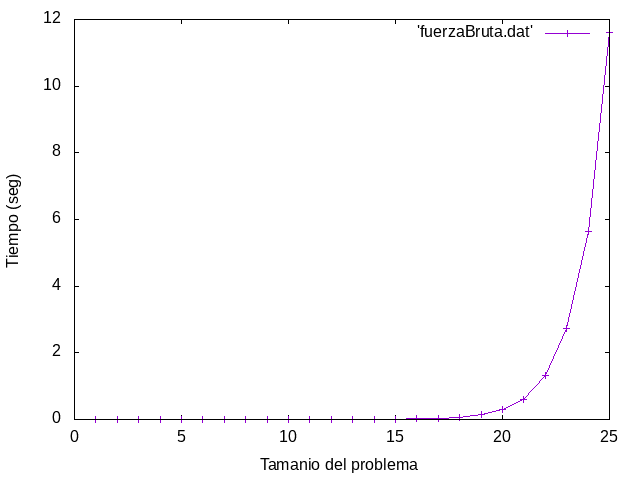
\includegraphics[scale=0.75]{fuerzaBruta.png}
	\caption{Fuerza bruta}
\end{figure}

\begin{figure}[H]
\centering
	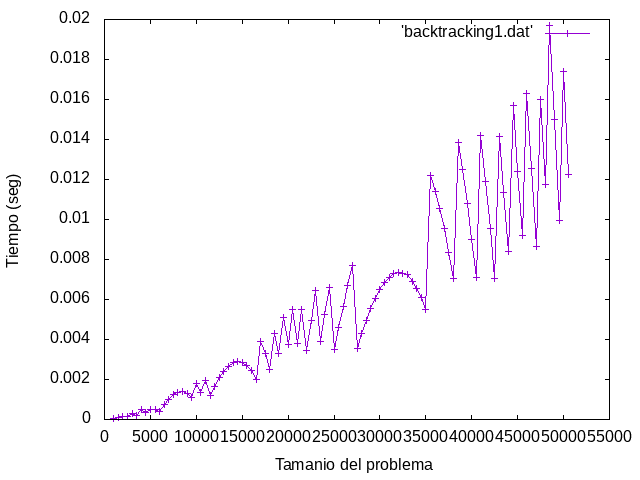
\includegraphics[scale=0.75]{backtracking1.png}
	\caption{Backtracking sin información}
\end{figure}

\begin{figure}[H]
\centering
	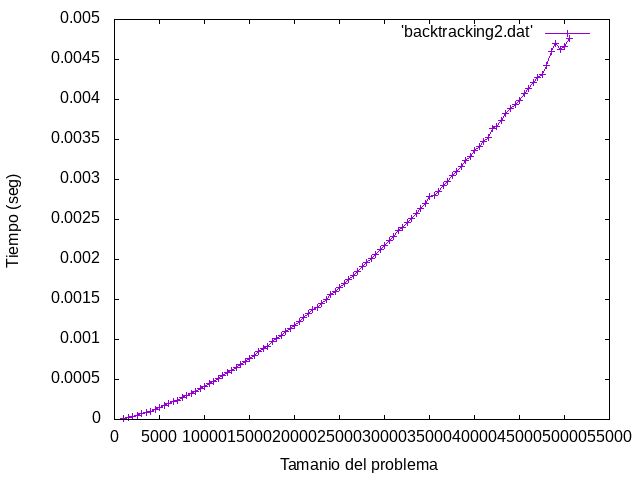
\includegraphics[scale=0.75]{backtracking2.png}
	\caption{Backtracking con información}
\end{figure}

\begin{figure}[H]
\centering
	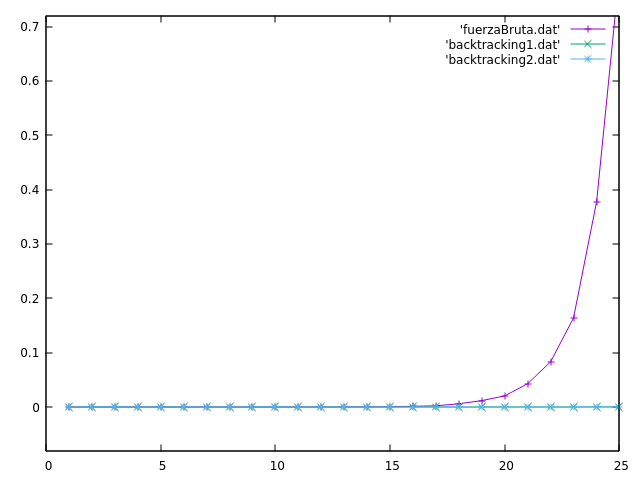
\includegraphics[scale=0.75]{todos.png}
	\caption{Comparativas entre algoritmos}
\end{figure}

\begin{figure}[H]
\centering
	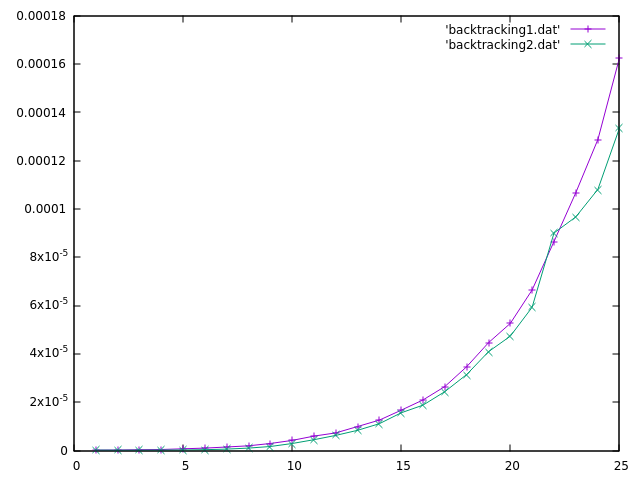
\includegraphics[scale=0.75]{ambos_backtracking.png}
	\caption{Comparativa entre algoritmos backtracking}
\end{figure}

\newpage

\section{Conclusiones}

Como hemos podido observar en las figuras anteriores, el algortimo fuerza bruta es nefasto. La eficiencia de este algoritmo es factorial lo cual da lugar a tiempos muy elevados.

Sin embargo con backtracking, conseguimos órdenes de eficiencia mucho menores por el simple hecho de realizar una comprobación de factibilidad. \\

Pero podemos afinar aún más; si almacenamos los datos que se evalúan en la función de factibilidad evitamos tener que calcularlos en cada iteración, transformando una función de orden de eficiencia lineal en una función de orden constante.

\section{Anexo: código fuente}
\cppcode{fuerzaBruta.cpp}
\captionof{figure}{Fuerza bruta}

\cppcode{backtracking1.cpp}
\captionof{figure}{Backtracking sin información}

\cppcode{backtracking2.cpp}
\captionof{figure}{Backtracking con información}

\script{all.sh}
\captionof{figure}{Ejecución de la práctica}

\script{individual.sh}
\captionof{figure}{Ejecución individual}

\script{gnuplot.sh}
\captionof{figure}{Generación de gráficas}

%%%%%%%%%%%%%%%%%%%%%%%%%%%%Fin del documento%%%%%%%%%%%%%%%%%%%%%%%%%%%%%%%%
\end{document}
